\section*{Question 9}
\textit{Plot the dissipation spectrum and verify if the dissipation computed from the spectrum matches the dissipation calculated using the gradients. Comment on the match between the two methods for the two datasets.}

\begin{figure}[!ht]
\centering
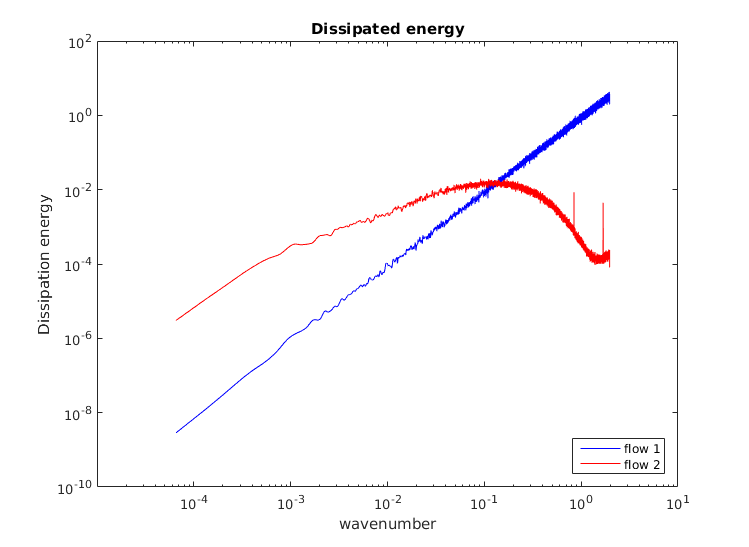
\includegraphics[scale=0.8]{./TEXT/esd-d.png}
\caption{Comparison between the energy spectral densities of both flow cases as they change with frequency for a window size of $20'000$ data points}
\label{esd-d}
\end{figure}

The dissipations for flow cases 1 and 2 are $4.886 \times 10^{-4}$ and $1.269 \times 10^{-6}$ respectively. These values are very different from those seen in section 3 by several orders of magnitude.